\chapter{Specifications and Design}

\section{User personas}

Person 1
\begin{itemize}
    \item Name: Feona
    \item Age: 17
    \item Relationship: Has a partner
    \item Location: Lives at home with parents
    \item School of study: Computer Science
    \item Frustrations: Having no easy place to ask questions about a module with other students.
    \item Hobbies: Computer Games, Art
    \item Preferred Channels: Discord, Reddit, WhatsApp
    \item Bio:
    \begin{itemize}
        \item Feona is a first-year student from the School of Computer Science who would like the ability to easily connect with other students on her course and find helpful resources for questions she has about specific activities as part of the modules she is taking
    \end{itemize}
\end{itemize}

Person 2
\begin{itemize}
    \item Name: John
    \item Age: 19
    \item Relationship: Single
    \item Location: Lives in a flat with room-mates
    \item School of study: English Language
    \item Frustrations: Fed up of the timetables not being updated correctly
    \item Hobbies: Reading, Clubbing, Rowing, writing short stories
    \item Preferred Channels: Instagram, WhatsApp, MS Teams
    \item Bio:
    \begin{itemize}
        \item John is a 19-year-old student studying English Language. They enjoy sitting for hours writing stories. They often forget to check their timetable and end up late for lectures, or when they do, a tutor may have changed the time, putting a message on the VLE and emailing students. Unfortunately, the timetables haven't been updated, and John rarely checks their emails, so they have turned up to lectures that don't exist on more than one occasion.
    \end{itemize}
\end{itemize}

\section{Requirements}

To define the actors in the requirements: "Student" is a Student, "Tutor" is a Tutor, and "User" is used when the requirement applies to both the Student and Tutor actors.

The requirements are broken into " must have, " " should have, " and "could have". Must have - the requirement must be present in the MVP. Should have - a desired requirement but not as important for proving the prototype's usability. Could have - requirements that are unlikely to make it into the final version of the prototype but should be included in further development if the application proves to work and be valuable to users.

\subsection{Functional requirements}
\subsubsection{MUST}

\begin{tabular}{|p{1cm}|p{13cm}|}
    \hline
        \textbf{ID} & \textbf{Requirement} \\
    \hline
    F-r1 &
    Users must be able to register an account login \\
    \hline
    F-r2 & 
    Students MUST be able to view upcoming lectures for that day (if available) \\
    \hline
    F-r3 &
    Students MUST be able to see the modules they are taking \\
    \hline
    F-r4 &
    Students MUST be able to see a list of modules relating to their year and school \\
    \hline
    F-r5 &
    Students MUST be able to post a question relating to a module \\
    \hline
    F-r6 &
    Students MUST be able to view information/resources relevant to a specific module \\
    \hline
    F-r7 &
    Students MUST be able to add resources to a module (pictures, pdfs) \\
    \hline
    F-r8 &
    Students MUST be able to comment on a question or post \\
    \hline
    F-r9 &
    Students MUST be able to message in a module’s group chat \\
    \hline
    F-r10 &
    Students MUST be able to view all available upcoming lectures for a specific module \\
    \hline
    F-r11 &
    Students MUST be able to subscribe to a module in their year and school \\
    \hline
    F-r12 &
    Students MUST be able to unsubscribe to a module \\
    \hline
    F-r13 &
    Users MUST be able to update their account info (Username, First name, etc) \\
    \hline
    F-r14 &
    Students MUST be able to see their home dashboard (user area home page) \\
    \hline
    F-r15 &
    Users MUST be able to log out of their account \\
    \hline
\end{tabular}

\subsubsection{SHOULD}

\begin{tabular}{|p{1cm}|p{13cm}|}
    \hline
        \textbf{ID} & \textbf{Requirement} \\
    \hline
    F-r16 &
    Students SHOULD be able to view lecture videos if linked \\
    \hline
    F-r17 &
    Students SHOULD be able to make notes on a lecture \\
    \hline
    F-r18 &
    Students SHOULD be able to create general notes \\
    \hline
    F-r19 &
    Students SHOULD be able to view and edit a created note \\
    \hline
    F-r20 &
    Students SHOULD be able to view a list of all the notes they’ve created \\
    \hline
    F-r21 &
    Students SHOULD be able to message another User directly \\
    \hline
    F-r22 &
    Students SHOULD be able to chat with users in real-time \\
    \hline
    F-r23 &
    Students SHOULD be able to review a module they are taking \\
    \hline
    F-r24 &
    Students SHOULD be able to see reviews of other modules in their school \\
    \hline
    F-r25 &
    Students SHOULD be able to view who posted a question \\
    \hline
    F-r26 &
    Students SHOULD be able to view the date-time a question was posted \\
    \hline
    F-r27 &
    Students SHOULD be able to view the date-time a question was edited \\
    \hline
    F-r28 &
    Students SHOULD be able to view who posted comments \\
    \hline
    F-r29 &
    Students SHOULD be able to view the date-time a comment was posted \\
    \hline
    F-r30 &
    Students SHOULD be able to view uploaded a module resource \\
    \hline
    F-r31 &
    Students SHOULD be able to view the date-time a module resource was posted/uploaded \\
    \hline
    F-r32 &
    Users SHOULD be able to update their public profile \\
    \hline
\end{tabular}

\subsubsection{COULD}

\begin{tabular}{|p{1cm}|p{13cm}|}
    \hline
        \textbf{ID} & \textbf{Requirement} \\
    \hline
    F-r33 &
    Students COULD be able to add another student as a friend \\
    \hline
    F-r34 &
    Students COULD be able to see their friends list \\
    \hline
    F-r35 &
    Students COULD be able to message a friend directly \\
    \hline
    F-r36 &
    Students COULD be able to add friends to a group chat \\
    \hline
    F-r37 &
    Tutors COULD be able to be assigned a student to a module \\
    \hline
    F-r38 &
    Students COULD be able to create a note against a friend \\
    \hline
    F-r39 &
    Students COULD be able to give a friend a nickname \\
    \hline
    F-r40 &
    Students COULD be able to invite another user to join the site \\
    \hline
    F-r41 &
    Tutors COULD be able to post polls for students to answer \\
    \hline
    F-r42 &
    Students COULD be able to use Markdown to type/format/edit posts, notes and comments \\
    \hline
    F-r43 &
    Users COULD be able to see which Tutor(s) are teaching a module \\
    \hline
    F-r44 &
    Users COULD be able to change between light mode and dark mode view \\
    \hline
    F-r45 &
    Users COULD use a Keyboard shortcut to send a message \\
    \hline
    F-r46 &
    Students COULD be able to view the modules they subscribed to in the past years (if applicable) \\
    \hline
\end{tabular}
    
\subsection{Non-functional requirements}
\subsubsection{MUST}

\begin{tabular}{|p{1cm}|p{13cm}|}
    \hline
        \textbf{ID} & \textbf{Requirement} \\
    \hline
    NF-r1 &
    When a lecture is added, the system MUST record who has performed this action and the date-time \\
    \hline
    NF-r2 &
    It MUST take a max of one click for a user to be able to navigate to their home page \\
    \hline
    NF-r3 &
    Once a new module has been added, a new message thread MUST be created and linked \\
    \hline
    NF-r4 &
    The system MUST create a new message thread once the first message is received from the current user, which has been sent to another user \\
    \hline
    NF-r5 &
    The system MUST add the user to the module's message thread after the user clicks the subscribes to the modules button \\
    \hline
    NF-r6 &
    A WebSocket connect MUST be established within 5 seconds of a user loading a single module page or a single message thread page \\
    \hline
    NF-r7 &
    The system MUST not allow a user to authenticate with incorrect details such as the wrong password \\
    \hline
    NF-r8 &
    It MUST not take a user more than one click to access a subscribed module page on a desktop or three clicks on a mobile device \\ 
    \hline
\end{tabular}    

\subsubsection{SHOULD}

\begin{tabular}{|p{1cm}|p{13cm}|}
    \hline
        \textbf{ID} & \textbf{Requirement} \\
    \hline
    NF-r9 &
    The system SHOULD try to retrieve og:tag information for a link when it is uploaded to the site \\
    \hline
    NF-r10 &
    OG:tags SHOULD load for a link (if available) when required for a page \\
    \hline
    NF-1 &
    A YouTube or Panopto video SHOULD not load/autoplay until it is clicked on by the user \\
    \hline
    NF-r12 &
    A YouTube or Panopto video MUST be embeddable onto the page when loaded \\
    \hline
    NF-r13 &
    HTTP long pulling SHOULD be established when a WebSocket connection fails if not due to internet disconnection \\
    \hline
\end{tabular}

\subsubsection{COULD}

\begin{tabular}{|p{1cm}|p{13cm}|}
    \hline
        \textbf{ID} & \textbf{Requirement} \\
    \hline
    NF-r14 &
    A page COULD load content as the user scrolls \\
    \hline
    NF-r15 &
    A note for a Student COULD autosave in the background every 15 seconds as they are editing \\
    \hline
    NF-r16 &
    A WebSocket COULD be established between the client (user’s computer) and the server after a user logins into the application \\
    \hline
\end{tabular}

\section{Database}
Throughout our course at university, we have had the opportunity to use multiple types of databases such as SQL, MongoDB and GraphDB. The prototype application uses an SQL-based (MySQL in RDS) for storing data using the following tables:

\begin{figure}[h]
    \includegraphics[scale=0.36]{images/database/database_diagram.png}
    \caption{Database design}
    \label{fig:my_label}
\end{figure}

\subsection{The tables}

\subsubsection{User}
The user table holds the essential information about a user of the application.

\subsubsection{University}
The University table is used to hold information about a university, such as name, location, etc.

\subsubsection{UniversitySchool}
The university school table is used for linking users, universities, and modules together. Defines the school the user is part of when they are linked to it and segregates the modules into the correct schools.

\subsubsection{UniversityYear}
The university year table is similar to the university school table but defines the year of study, e.g. Year 1.

\subsubsection{Module}
The module table has the main information about a module and is used to connect anything for a specific module, such as lectures, resources and notes.

\subsubsection{ModuleLecture}
The module lecture table is used by a tutor to define upcoming lectures, whether they are in person or online. It allows a tutor to link Zoom/MS Teams link for online lectures and a quiz link to Mentimeter/Kahoot for improving student engagement. This allows a student quick access to the information they need to know for a lecture in one easy place.

\subsubsection{ModuleQuestion}
The module question table is used for a student to post questions and link them to a module.

\subsubsection{ModuleQuestionComment}

The module question comment table links to the module question table and allows users to post their replies to a question.

\subsubsection{Image}
The image table is used to hold information about images uploaded to the application by users. This holds the location of the image, title and description of the image added by users.

\subsubsection{Document}
The document table is similar to the image table and holds the same information structures but is separated to split out images and documents for organisation purposes and to allow the image table to be used for image-specific purposes in the future.

\subsubsection{ModuleResource}
The module resource table is used to link a row in the image or document table to a module.

\subsubsection{ModuleReview}
The module review table is used to hold the reviews from students on a module. This table didn't end up getting used in the prototype but is left to add it in the future.

\subsubsection{ModuleSubscription}
The module subscription table is used to link a user to a module. When a user is subscribed to a module, information and intractability with the module become possible. It allows users to choose modules they want to see information for on their home page and sidebar.

\subsubsection{PublicProfile}
The public profile table is used for a user to add information they want to be seen publicly by other users. For the prototype, only a user bio is added, but it allows for future expansions, such as allowing a user to add their interest/hobbies, pronouns, etc. It also means that only the needed essential information for a user is accessed in the user table, which is accessed almost every time a user interacts with the application. This will allow the application to scale better if and when it expands.

\subsubsection{PublicPost}
The public post table is similar to the module question table but is used when a user wants to post things publicly for other users not subscribed to a specific module. This would be left to the user to decide what to post but would be expected to be used for leisure purposes, not university or study-specific purposes.

\subsubsection{PublicPostComment}
The public post comment table is similar to the module question comment table but links to a public post instead.

\subsubsection{Message}
The massage table is used to hold the contents and metadata of a message a user sends in the real-time chat sections.

\subsubsection{MessageThread}
The message thread table is used to link a collection of messages into one stream (conversation). It allows a user to click on a chat and only see the message specific to that conversation.

\subsubsection{Note}
The note table is used to hold the notes a user creates. This can be linked to a module to see the note's purpose easily.

\section{Wire-framing}

To get an idea for the design, wireframes were created on paper. The designs have been annotated to point out and denote the different sections, such as pointing out the header/navigation. As the application is getting built, it will change, but these designs should give an example of how the application could look for some of the sections.

\subsection{User home}
\begin{figure}[H]
    \centering
    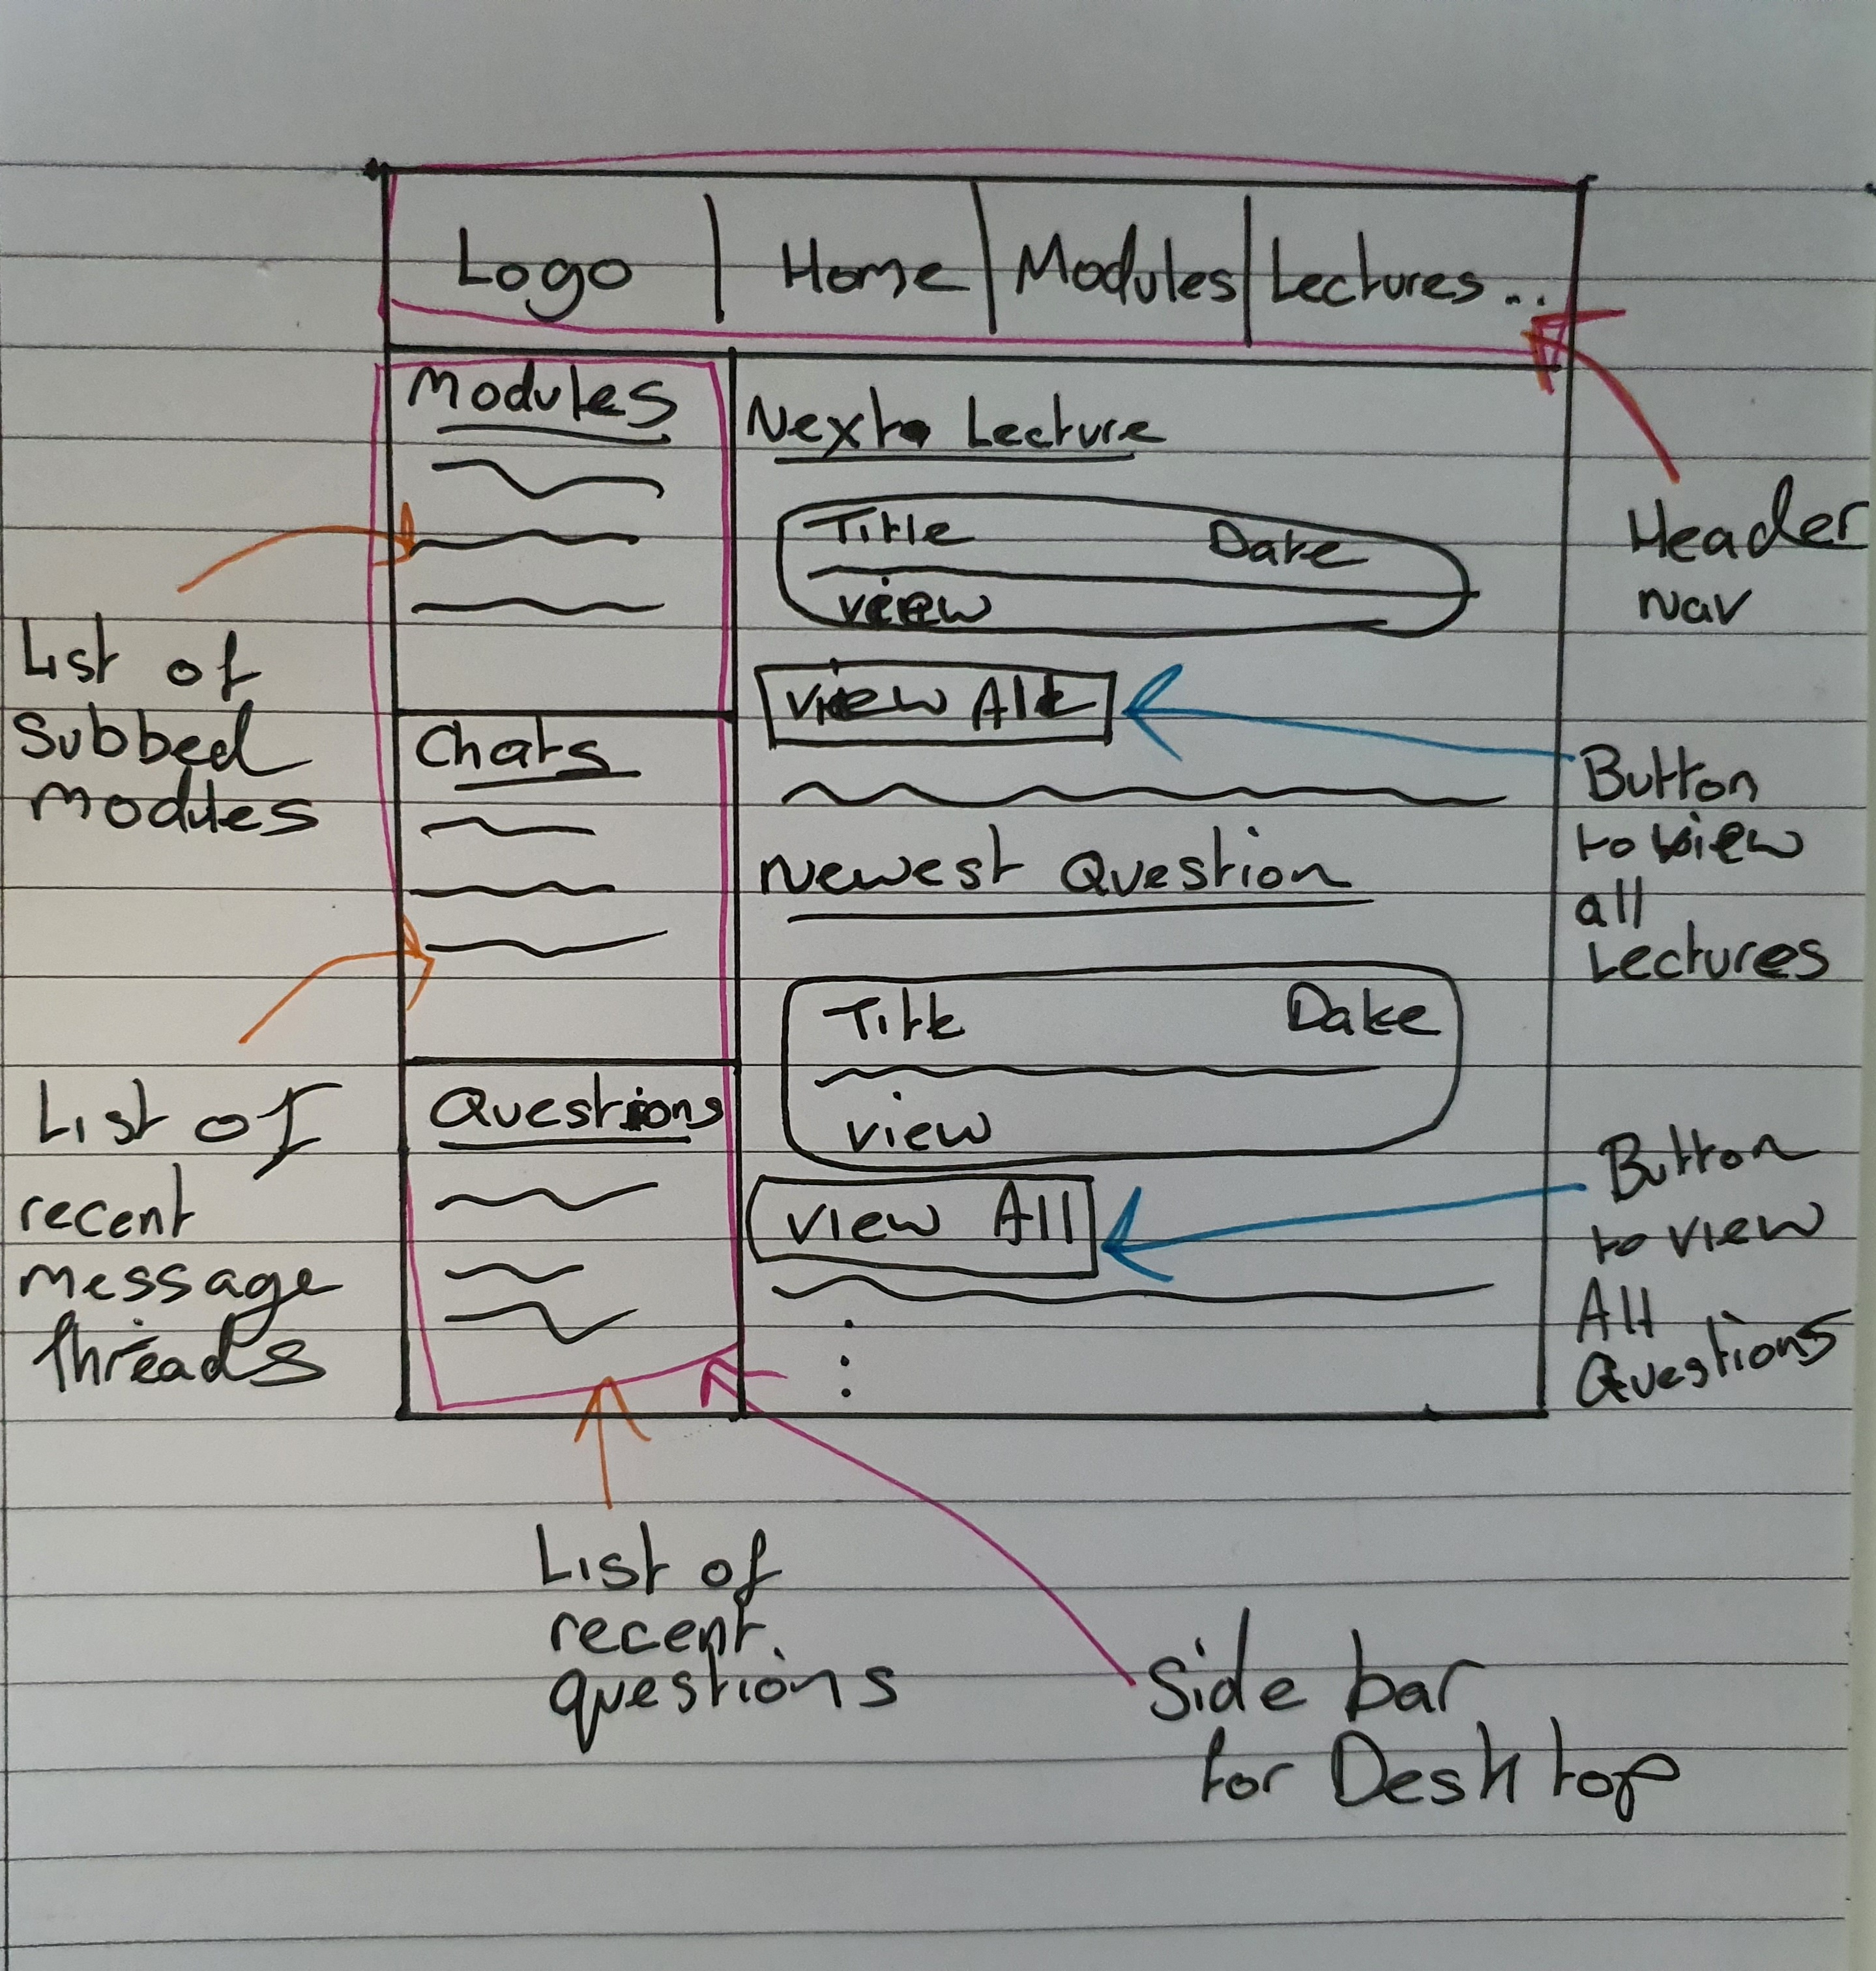
\includegraphics[scale=0.14]{images/wireframe/user_home.jpg}
    \caption{User home page wireframe}
    \label{fig:my_label}
\end{figure}
This design is to show what the user will first see upon logging into the application. It shows the top part of the page (above the fold).

\subsection{Lectures}
\begin{figure}[H]
    \centering
    \includegraphics[scale=0.15]{images/wireframe/lectures.jpg}
    \caption{User lecture list page wireframe}
    \label{fig:my_label}
\end{figure}
This design is to show an example of what a page with different list items will look like, for example, the list of questions, list of lectures, list of all modules, etc. 

\subsection{Mobile}
\begin{figure}[H]
    \centering
    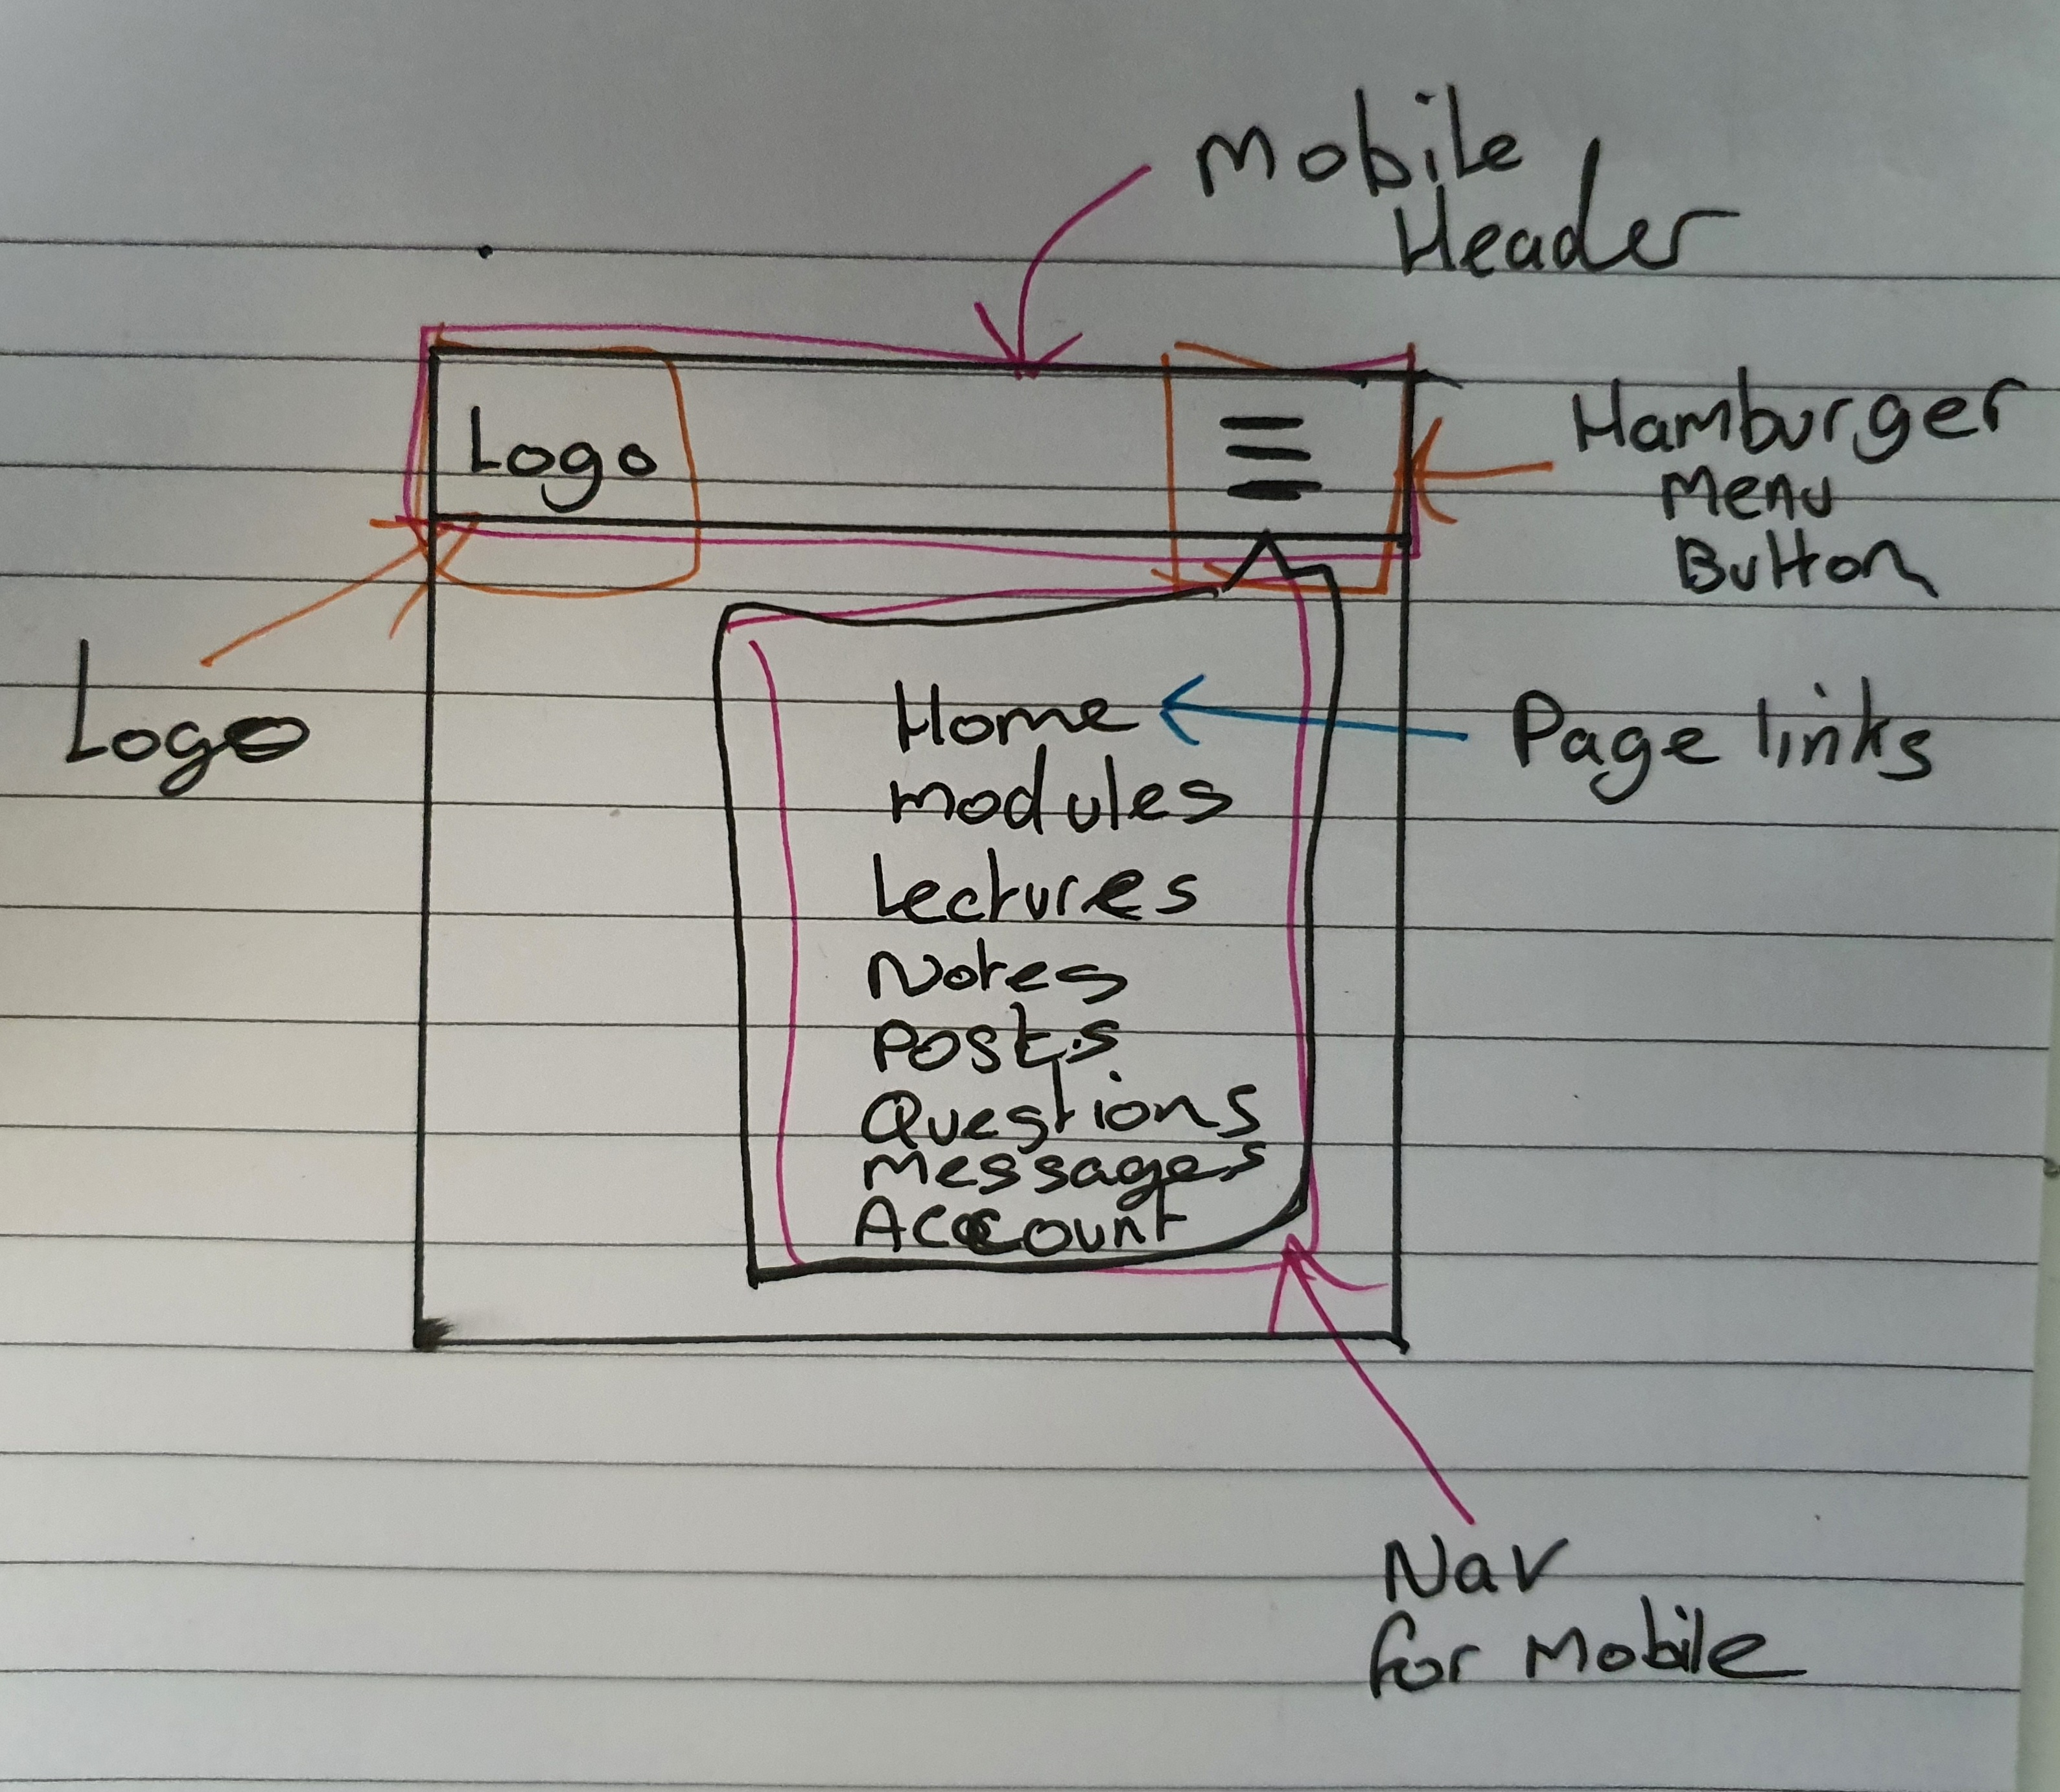
\includegraphics[scale=0.13]{images/wireframe/mobile.jpg}
    \caption{Mobile example wireframe}
    \label{fig:my_label}
\end{figure}

This is an example of how the application could look on a mobile device. It doesn't show any specific page but instead how the mobile menu would differ. The navigation collapses into a hamburger menu and drops down when the user taps on the button.

\section{Use cases}

\subsection{Lectures}

\begin{figure}[H]
    \centering
    \includegraphics[scale=0.45]{images/use cases/lectures.png}
    \caption{Lectures use case diagram}
    \label{fig:my_label}
\end{figure}

Users have different relationships with lectures depending on which actors they are. Students can view the list of lectures and click to view more information about a lecture. Tutors can do this too, but they also have the ability to create and delete lectures.

\subsection{Messages}

\begin{figure}[H]
    \centering
    \includegraphics[scale=0.45]{images/use cases/messages.png}
    \caption{Message  use case diagram}
    \label{fig:my_label}
\end{figure}

All users have the ability to interact with each other through Real-time messaging, which is accessible from the messages section and the module page for module chats. Users can view messages and threads they are linked to and send a message to the thread. A thread may contain two users for direct messaging or many users for module chats.

\subsection{Module}
 
\begin{figure}[H]
    \centering
    \includegraphics[scale=0.36]{images/use cases/module.png}
    \caption{Module use case diagram}
    \label{fig:my_label}
\end{figure}

On a single module page, there are a lot of the functions from above, viewing lectures and real-time messaging. There is also the viewing of module resources, other uses who are subscribed to the module, module questions and about the module. A student can click to create a student resource, whereas a tutor can click to create a tutor resource or to create a lecture.

\subsection{Notes}

\begin{figure}[H]
    \centering
    \includegraphics[scale=0.45]{images/use cases/notes.png}
    \caption{Notes use case diagram}
    \label{fig:my_label}
\end{figure}

Notes are not restricted to use, but students, as a tutor, may decide to keep their notes for a lecture in the application to keep them in one place. For this reason, all users can view, create and edit notes.

\section{Wireframes}

To get an idea for the design, wireframes were created on paper. The designs have been annotated to point out and denote the different sections, such as pointing out the header/navigation. As the application is getting built, it will change, but these designs should give an example of how the application could look for some of the sections.

\subsection{User home}
\begin{figure}[H]
    \centering
    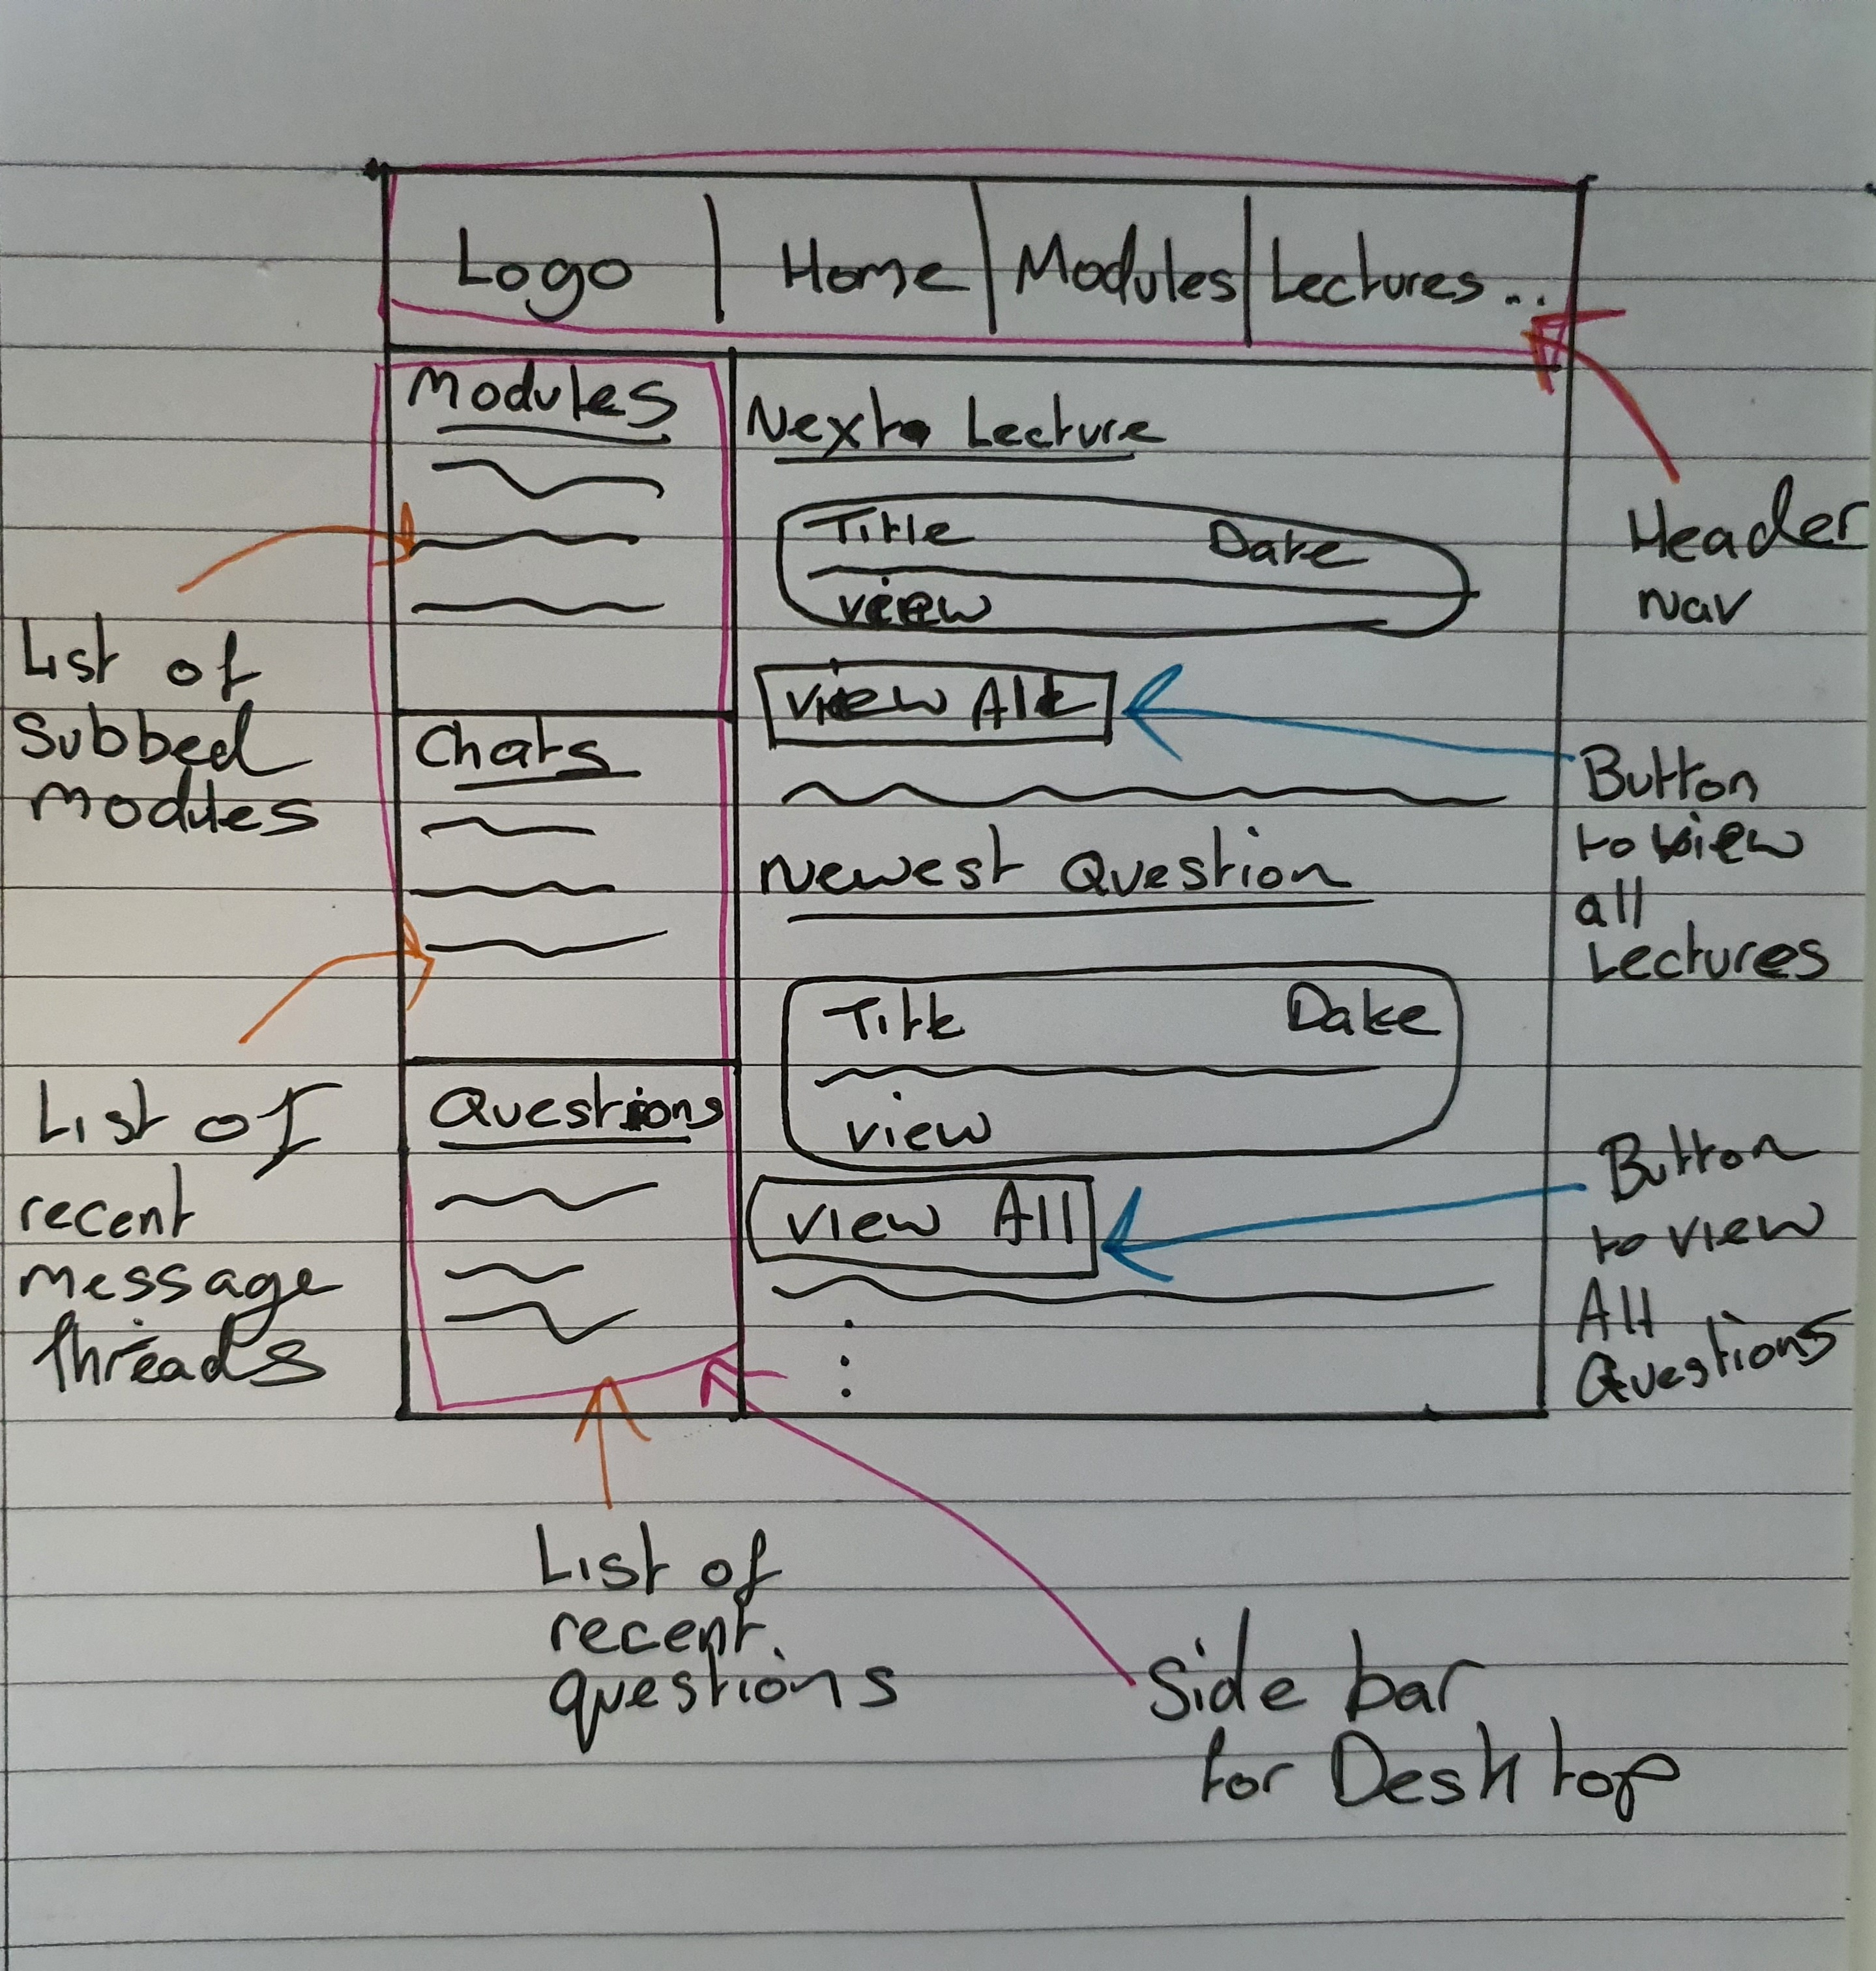
\includegraphics[scale=0.15]{images/wireframe/user_home.jpg}
    \caption{User home page wireframe}
    \label{fig:my_label}
\end{figure}
This design is to show what the user will first see upon logging into the application. It shows the top part of the page (above the fold).

\subsection{Lectures}
\begin{figure}[H]
    \centering
    \includegraphics[scale=0.15]{images/wireframe/lectures.jpg}
    \caption{User lecture list page wireframe}
    \label{fig:my_label}
\end{figure}
This design is to show an example of what a page with different list items will look like, for example, the list of questions, list of lectures, list of all modules, etc. 

\subsection{Mobile}
\begin{figure}[H]
    \centering
    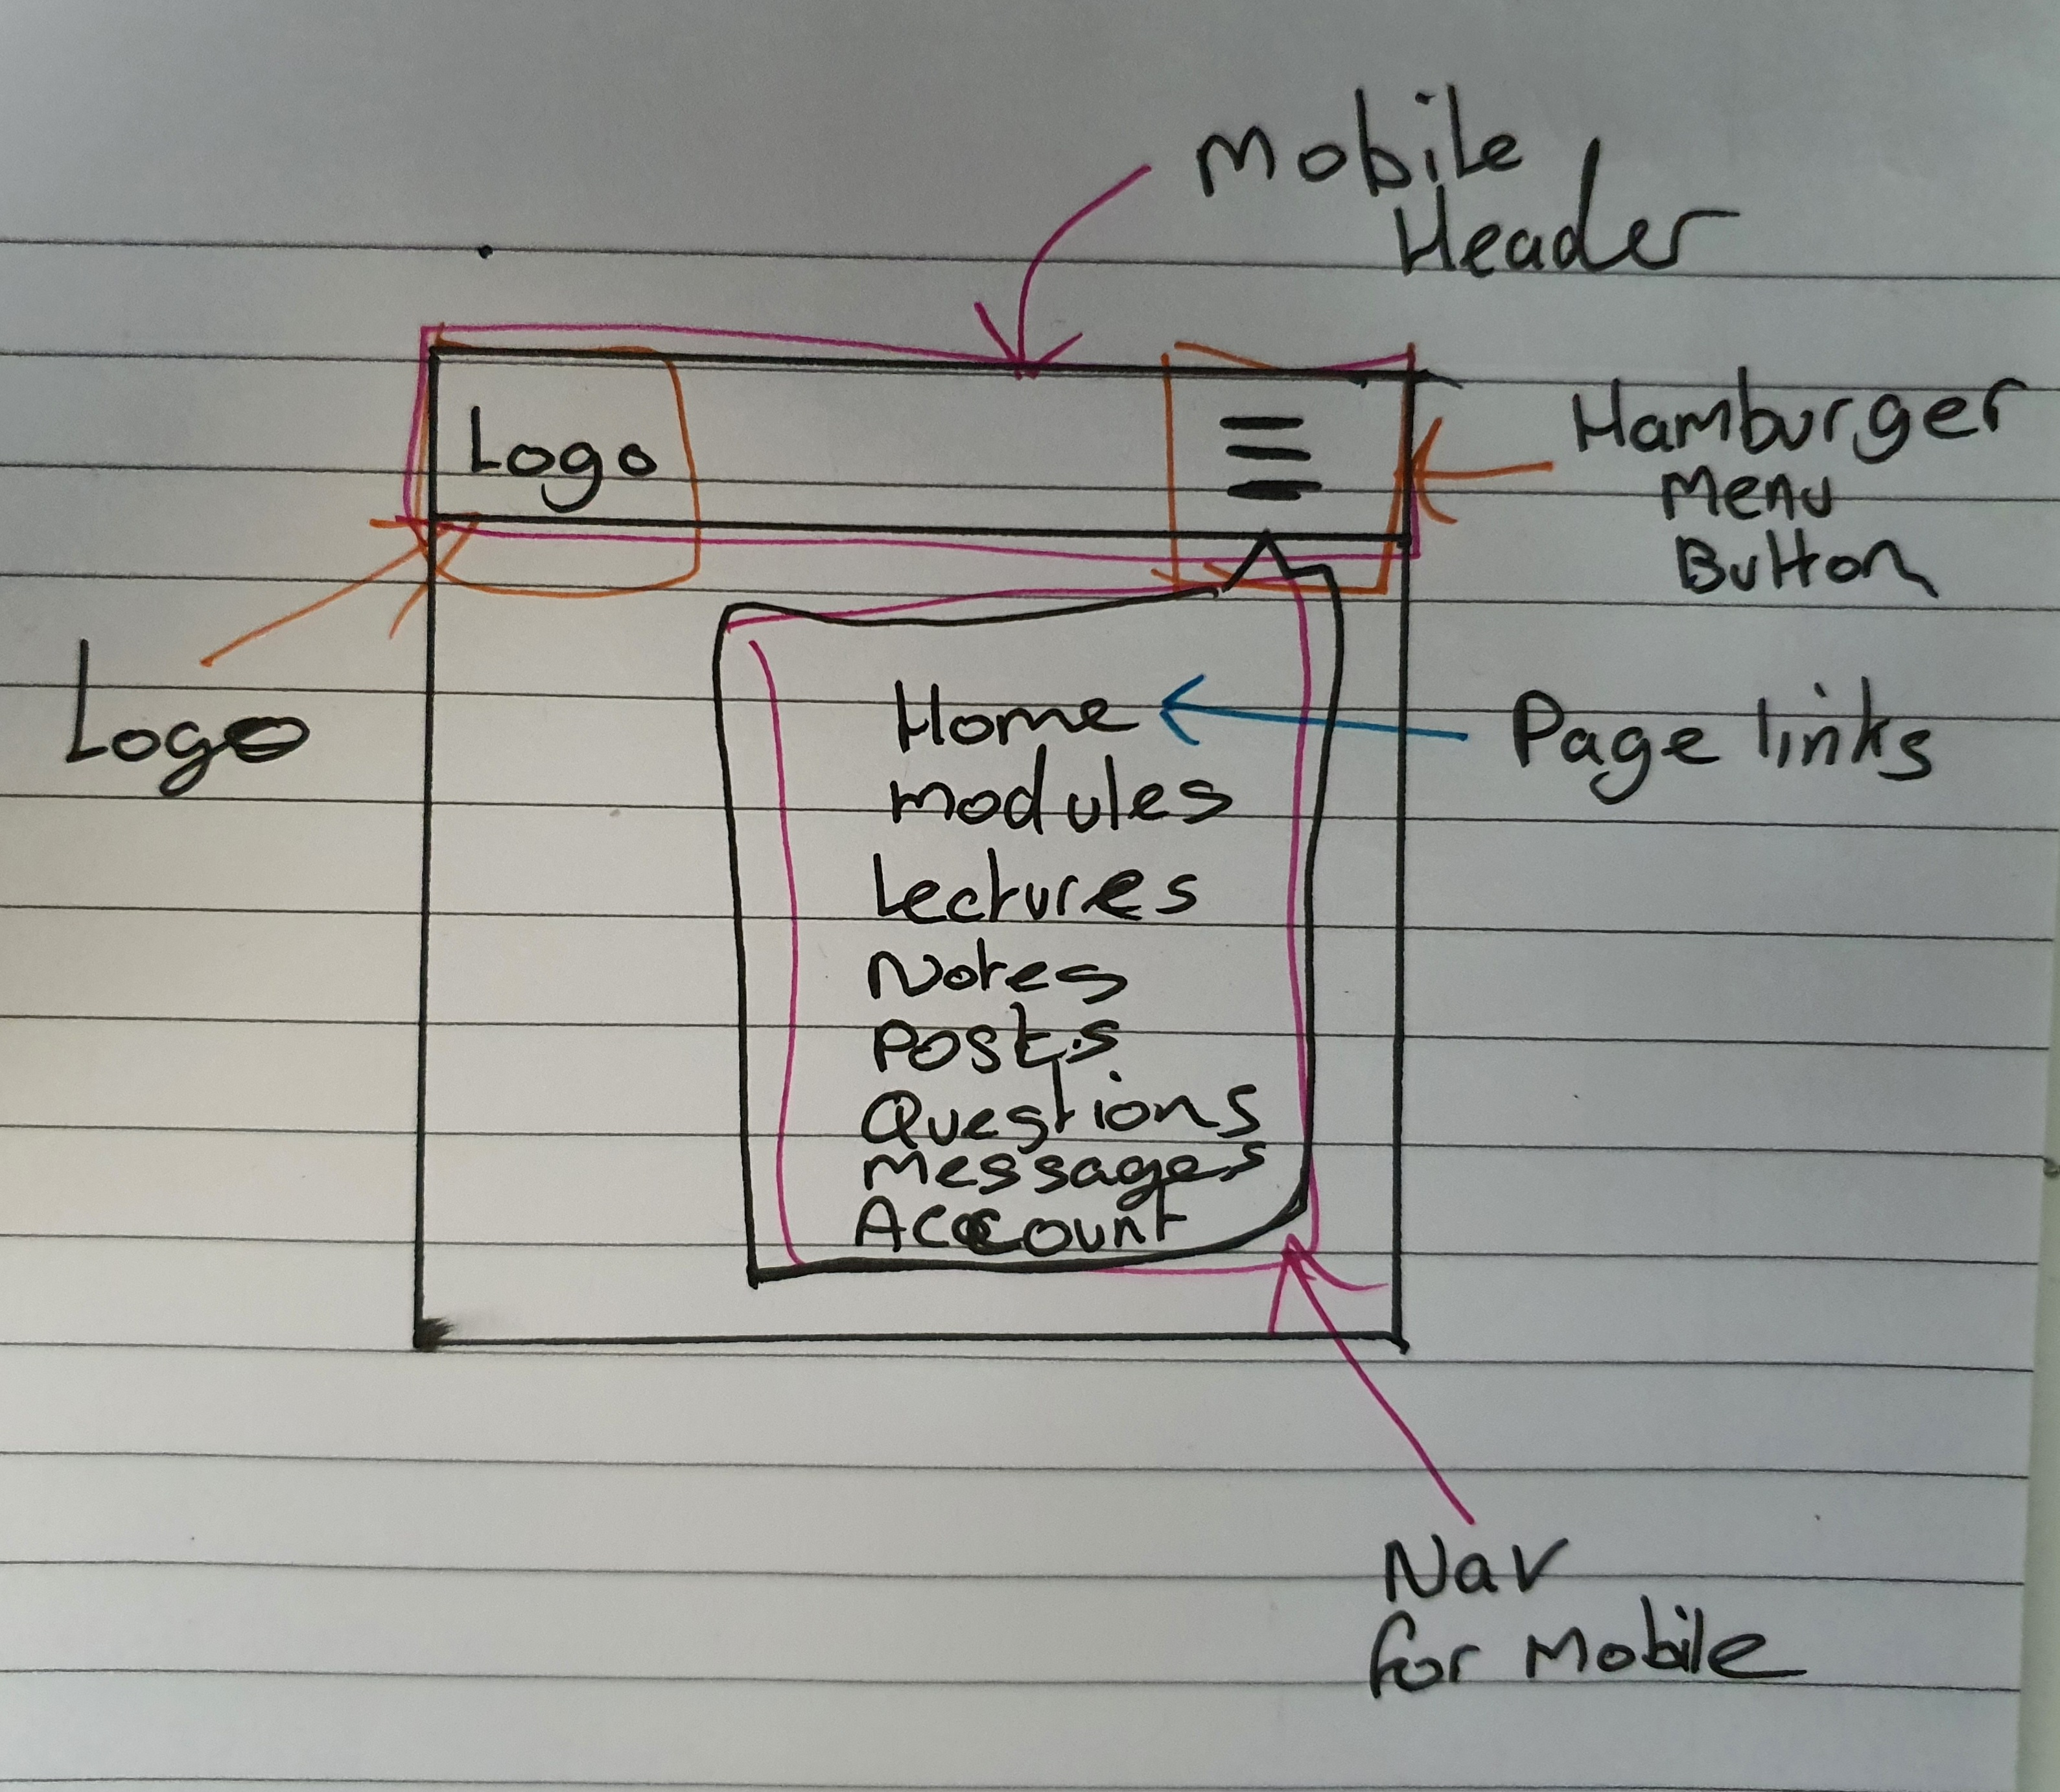
\includegraphics[scale=0.15]{images/wireframe/mobile.jpg}
    \caption{Mobile example wireframe}
    \label{fig:my_label}
\end{figure}

This is an example of how the application could look on a mobile device. It doesn't show any specific page but instead how the mobile menu would differ. The navigation collapses into a hamburger menu and drops down when the user taps on the button.